\documentclass[letterpaper,12pt]{article}

\title{Título del documento}
\author{Rodrigo Segura Moreno}
\date {\today }

%% Matemáticas
\usepackage{amsmath}
\usepackage{amssymb}

\usepackage{upgreek} % Greek alphabet

\usepackage{hyperref} % URL
\usepackage{xcolor} % Colores

\usepackage{changepage} % Margins

\usepackage[letterpaper, margin=1 in]{geometry}
\usepackage{graphicx}

\usepackage{gensymb} % Generic symbols for both text and math mode.

\usepackage{systeme}

\begin{document}
	
	\thispagestyle{empty}
	
	\begin{figure}
		\minipage{0.76\textwidth}
			
\includegraphics[ width = 1.65in,height=1.65in ]{FC.jpg}
		\endminipage
		\minipage{0.32\textwidth}
			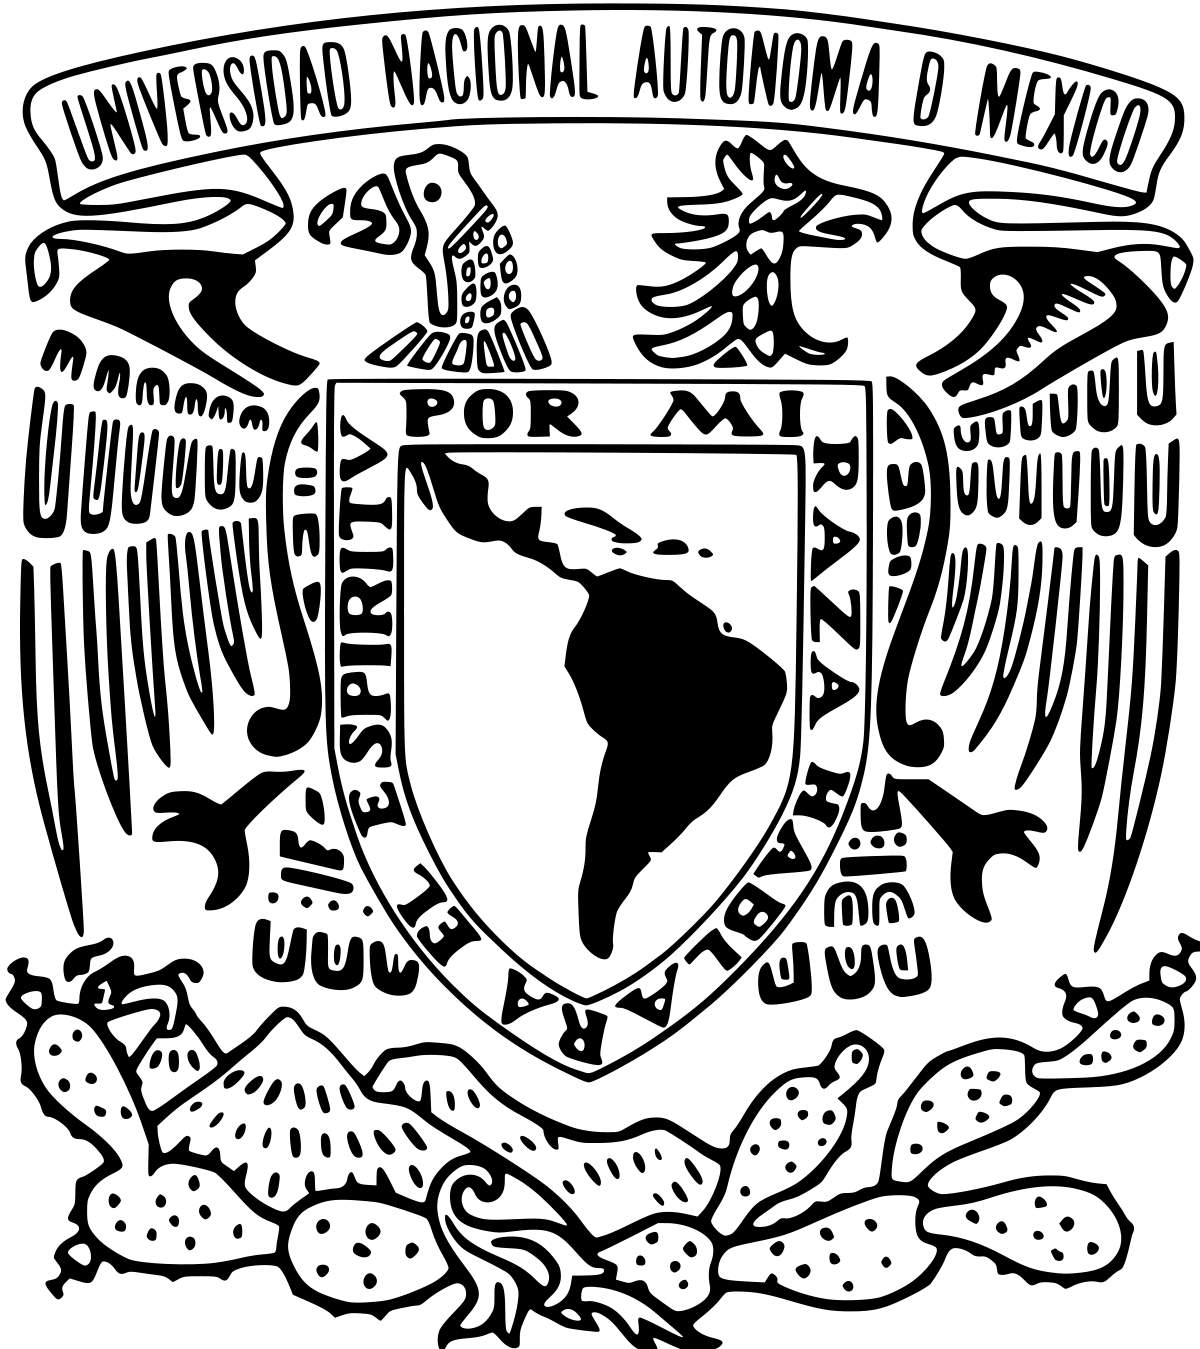
\includegraphics[ width = 1.25in,height=1.25in ]{UNAM.png}
		\endminipage
	\end{figure}

	\vspace{0.5cm}
	
	\begin{center}
		\textbf{\large Universidad Nacional Autónoma de México \\}
		\textbf{\large Facultad de Ciencias} \\
		
		\vspace{0.7cm}
		
		{\large  \textbf{Computación} \\}
		\textbf{Grupo:} 8093\\
		Dr. Sergio Antonio Alcalá Corona\\
		Fis. Sergio Ángel Sánchez Chávez
		
		\vspace{0.5cm}
		
		{\large Tarea Programa en LaTeX \\}
		11 de diciembre de 2020
		
		\vspace{0.7cm}
		
		Rodrigo Segura Moreno \\
		
	\end{center}

	\vspace{5pt}
	\hrule
	\vspace{3em}

	El programa a desarrollar en Python deberá resolver sistemas de dos ecuaciones y dos incógnitas. Para ejemplificar considere que se tiene un sistema de la siguiente forma
	$$
		\begin{cases}
			ax + by = c \\
			dx + ey = f \\
		\end{cases}
	$$

	\noindent donde:
	\begin{itemize}
		\item $ x $ y $ y $ son variables
		\item $ a,b,d,e $ son coeficientes
		\item $ c $ y $ f $ son constantes.
	\end{itemize}

	El programa deberá aceptar cualesquiera valores que el usuario establezca de $ a,b,c,d,e $ y $ f \in \mathbb{R} $ y encontrar las incógnitas que satisfacen al sistema de ecuaciones.
	
\end{document}